% ============================ Part 3: Prompting & ICL ============================
\section{Part 3 $\cdot$ Prompting \& ICL}
\partslide{3}{Prompting \& in-context learning}{learning by example}

\begin{frame}{A pretrained LM continues text; prompting designs the input}
\begin{columns}[T]
\begin{column}{0.5\textwidth}
\begin{itemize}\setlength{\itemsep}{6pt}
  \item A \textbf{prompt} is the text we hand the model; its only job is to continue it.
  \item \textbf{Prompting} = write the prompt so that the \emph{most likely continuation} is the answer we want.
  \item \textbf{Zero-shot:} a task description, no examples.
  \item No training, no gradient, no change to $\theta$.
\end{itemize}
\end{column}
\begin{column}{0.48\textwidth}
\textbf{Sentiment analysis by continuation}
\begin{userbox}Review: \emph{The food was cold and the service painfully slow.}\\ Sentiment:\end{userbox}
\begin{modelbox}negative\end{modelbox}
\textbf{Question answering by continuation}
\begin{userbox}Q: Who wrote \emph{Hamlet}?\\ A:\end{userbox}
\begin{modelbox}William Shakespeare\end{modelbox}
\end{column}
\end{columns}
\end{frame}

\begin{frame}{In-context learning: learning from examples with frozen weights}
\begin{columns}[T]
\begin{column}{0.52\textwidth}
\centering
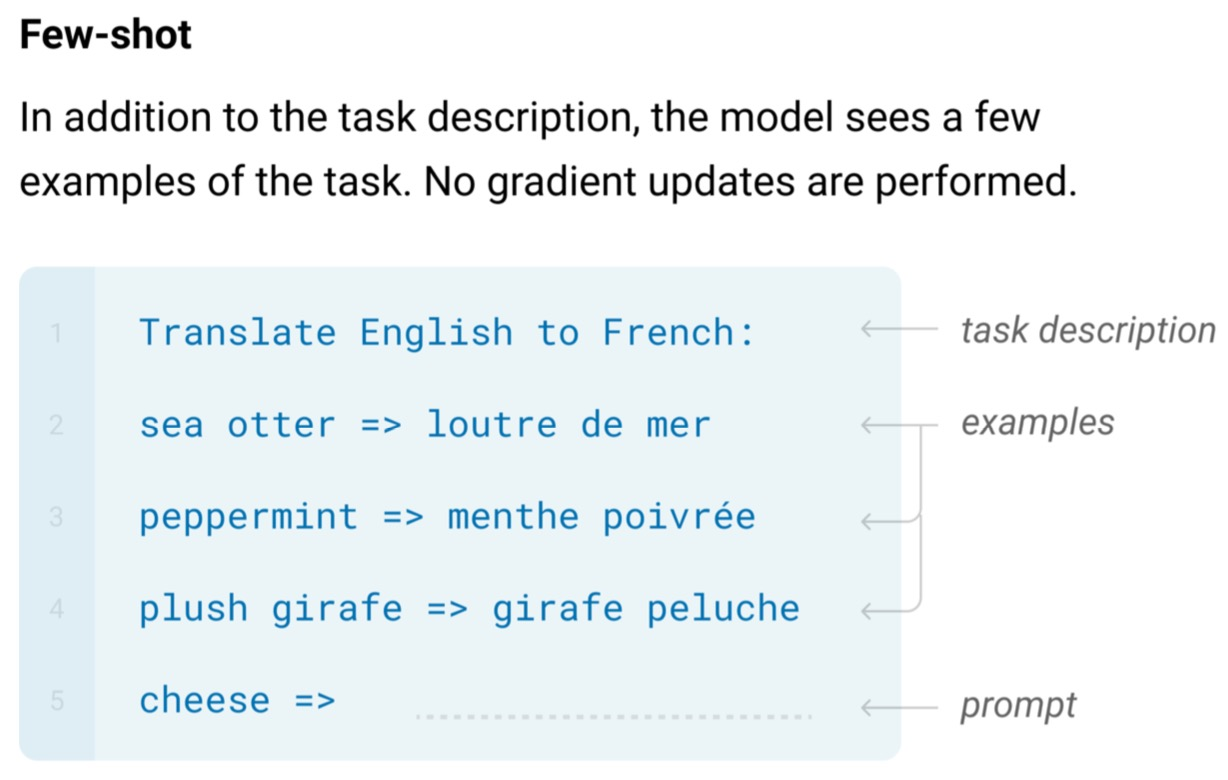
\includegraphics[width=\textwidth]{figs/gpt3_icl.png}\\[2pt]
\scriptsize Few-shot prompting in the GPT-3 paper (2020).
\end{column}
\begin{column}{0.46\textwidth}
\begin{itemize}\setlength{\itemsep}{6pt}
  \item \textbf{Few-shot / in-context learning (ICL):} put $k$ input$\to$output examples in the prompt; the model produces the output for a new input.
  \item Appears at scale (GPT-3): bigger models get much better at it.
  \item \textbf{No parameter update.} The ``learning'' happens inside one forward pass.
\end{itemize}
\end{column}
\end{columns}
\vspace{6pt}
\callback{everything so far}{Every algorithm in this course learns by changing weights with gradient steps. ICL adapts \emc{without touching the weights}. How it does so is still debated: one line of work argues that attention implicitly performs a form of gradient descent on the examples inside the forward pass (\href{https://arxiv.org/abs/2212.07677}{von Oswald et al., 2023}; \href{https://arxiv.org/abs/2212.10559}{Dai et al., 2023}).}
\end{frame}

\begin{frame}{In-context learning, live: two examples change the answer}
\begin{columns}[T]
\begin{column}{0.49\textwidth}
\textbf{Demo 1: letter manipulation}
\begin{userbox}Swap the second and the penultimate letter of the following word: \texttt{pothyn}\end{userbox}
\begin{modelbox}[badred]\texttt{pohtyn} \quad \bad\end{modelbox}
\begin{userbox}Directly answer the last one (swapping the second and the penultimate letter):\\ \texttt{tarehd} $\to$ \texttt{thread}, \; \texttt{revir} $\to$ \texttt{river}, \; \texttt{pothyn} $\to$\end{userbox}
\begin{modelbox}[okgreen]\texttt{python} \quad \ok\end{modelbox}
\end{column}
\begin{column}{0.49\textwidth}
\textbf{Demo 2: counting letters}
\begin{userbox}How many `r' letters are there in the following word: ``strawberry''?\end{userbox}
\begin{modelbox}[badred]There are 2 `r' letters in ``strawberry''. \quad \bad\end{modelbox}
\begin{userbox}Count how many `r' letters are there in the following words:\\ ``red'': 1, \; ``roar'': 2, \; ``strawberry'':\end{userbox}
\begin{modelbox}[okgreen]3 \quad \ok\end{modelbox}
\end{column}
\end{columns}
\vspace{6pt}
\centering\small\gray{Why is this hard at all? The model sees \emph{tokens}, not letters. The examples do more than fix the output format: they steer the model toward the right computation, working letter by letter. A first step toward chain-of-thought (next slide).}
\end{frame}

\begin{frame}{Chain-of-thought prompting: ask for the steps}
\begin{columns}[T]
\begin{column}{0.6\textwidth}
\centering
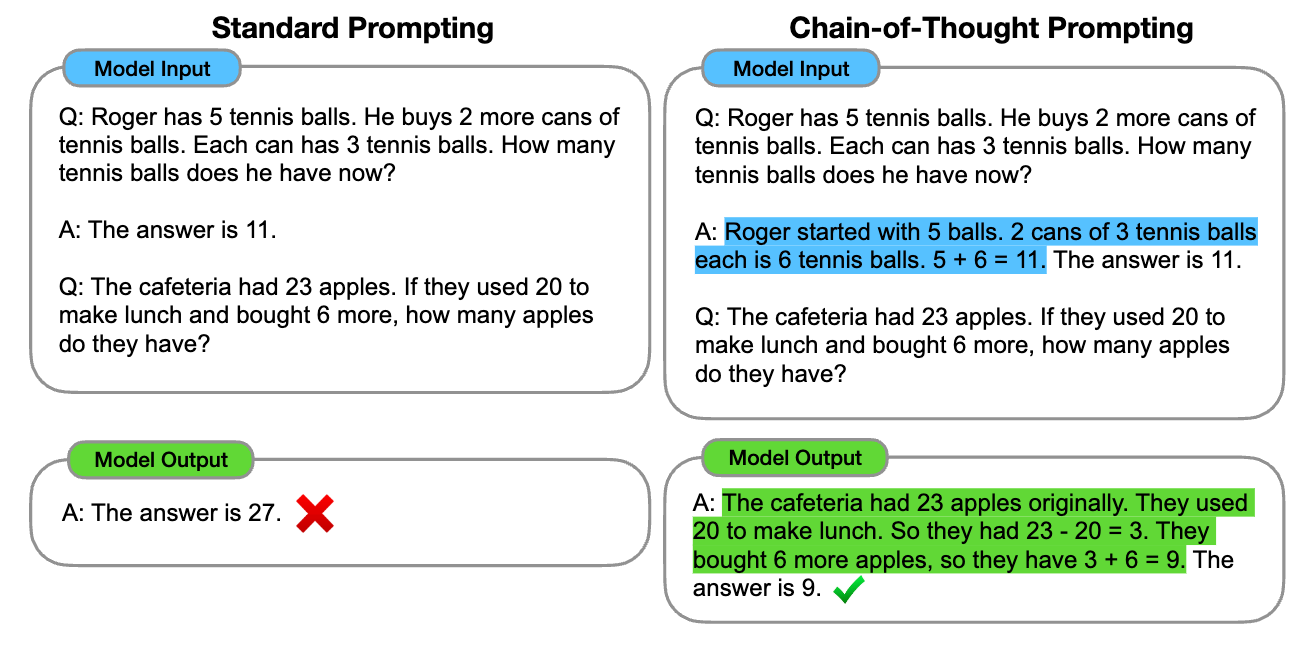
\includegraphics[width=\textwidth]{figs/cot_vs_standard.png}\\[2pt]
\scriptsize Few-shot chain-of-thought (\href{https://arxiv.org/abs/2201.11903}{Wei et al., 2022}).
\end{column}
\begin{column}{0.38\textwidth}
\begin{itemize}\setlength{\itemsep}{6pt}
  \item Show (or just request) \textbf{intermediate reasoning steps} before the final answer.
  \item Large gains on math and logic problems.
  \item Why it helps: one forward pass does a \textbf{fixed amount of computation} per token. Writing the steps out puts each intermediate result back into the input, so the model gets a \emc{scratchpad} and, in effect, more steps of computation.
\end{itemize}
\end{column}
\end{columns}
\end{frame}

\begin{frame}{Chain-of-thought works zero-shot --- and mostly for large models}
\begin{columns}[T]
\begin{column}{0.5\textwidth}
\centering
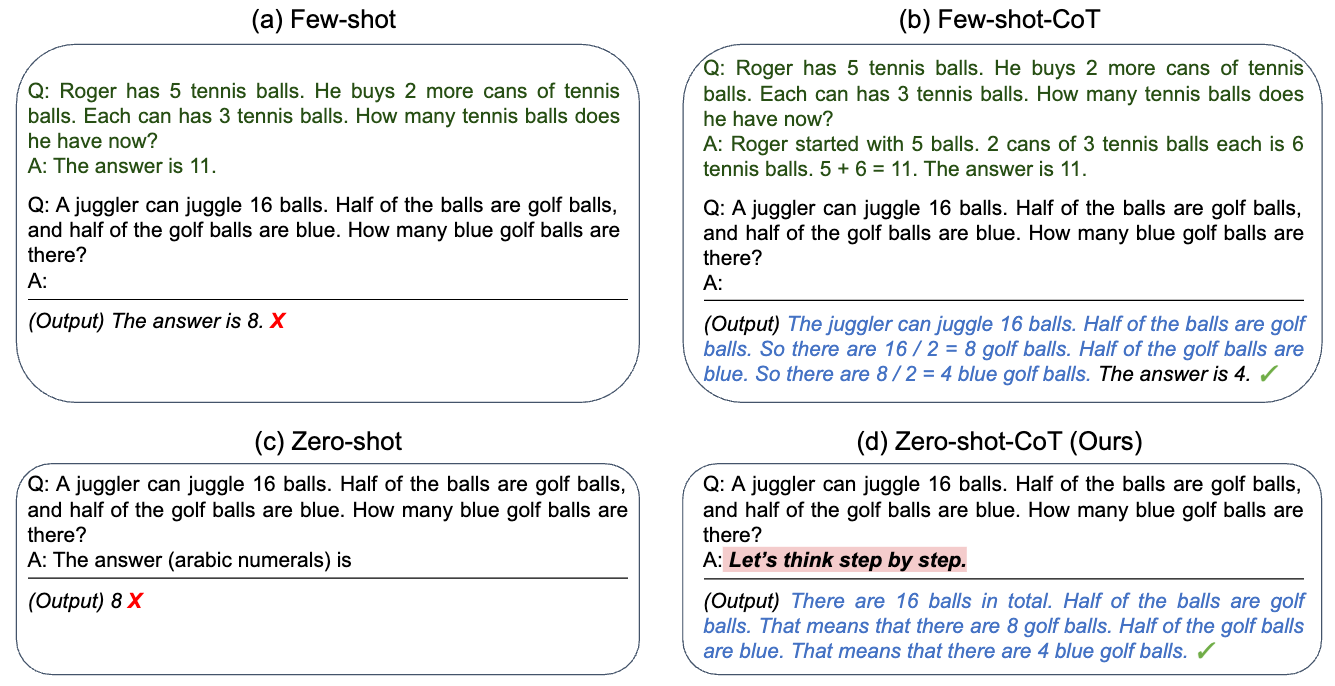
\includegraphics[width=\textwidth]{figs/zero_shot_cot.png}\\[2pt]
\scriptsize Just append \emph{``Let's think step by step.''} (Kojima et al., 2022).
\end{column}
\begin{column}{0.48\textwidth}
\centering
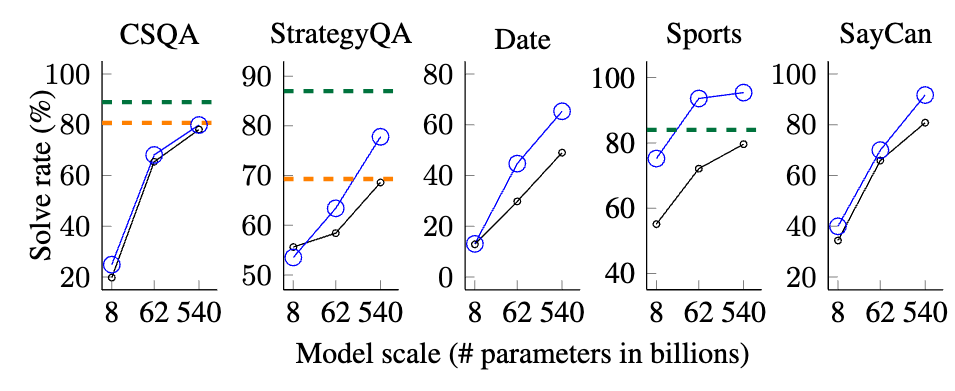
\includegraphics[width=\textwidth]{figs/cot_perf.png}\\[2pt]
\scriptsize CoT helps once models are large enough; small models produce fluent but wrong chains.
\end{column}
\end{columns}
\vspace{8pt}
\keybox{Foreshadowing Part 7: reasoning models (o1, R1) learn to produce long chains of thought \emph{on their own}, via reinforcement learning.}
\end{frame}

\begin{frame}{The limits of prompting}
\begin{columns}[T]
\begin{column}{0.52\textwidth}
\begin{itemize}\setlength{\itemsep}{6pt}
  \item \textbf{Fragile:} results depend on wording and example choice.
  \item \textbf{Expensive at use time:} examples must be re-sent with every query.
  \item \textbf{A base model is not trying to help you:} it continues text (Part 1 demo).
  \item \textbf{Nothing persists:} prompting cannot permanently add a skill, a style, or a safety rule.
\end{itemize}
\end{column}
\begin{column}{0.46\textwidth}
\keybox{To change what the model does \emph{by default}, change $\theta$.\\[6pt]
\textbf{Part 4:} supervised fine-tuning --- show it what good responses look like.\\[4pt]
\textbf{Parts 5--7:} reinforcement learning --- tell it how good its own responses were.}
\end{column}
\end{columns}
\end{frame}
